\documentclass[aspectratio=169]{beamer}
% \documentclass[aspectratio=169,handout]{beamer}

% Trying to use notes on separate page
% \documentclass[aspectratio=169,notes]{beamer}       % print frame + notes
% \documentclass[notes=only]{beamer}   % only notes
% \documentclass{beamer}              % only frames
%\usepackage{pgfpages}
%\setbeameroption{show notes}
%\setbeameroption{show notes on second screen=right}
%

%\setbeamercovered{transparent}

\usetheme[titleformat=regular%
,numbering=fraction% use slide numbers
]{metropolis}
\metroset{%
  progressbar=foot,%
  %background=dark,
  block=fill
}
\only<handout>{\metroset{sectionpage=none}}
\only<handout>{\usecolortheme{dove}}
\usepackage{appendixnumberbeamer} % separate appendix
\usepackage[citestyle=authortitle,sorting=none]{biblatex}
\setbeamerfont{footnote}{size=\tiny}
\addbibresource{mae.bib}

% multimedia in beamer presentations
\usepackage{multimedia}

% adding some better facilities to latex such as proper booleans
\usepackage{etoolbox}

% Unicode math symbols for XeLaTeX
\usepackage{mathrsfs}

% standard math packages
\usepackage{amssymb}
\usepackage{amsthm}
\usepackage{amsmath}
\usepackage{amstext}
\usepackage{mathabx}
\usepackage{stmaryrd}
% math tools for amsmath
\usepackage{mathtools}

\usepackage{proof}

\usepackage{pgfpages}

\usepackage{listings}
\usepackage{xcolor}

% subfigures, subfloats
\usepackage{subcaption}

% for multiinclude
\usepackage{xmpmulti}

% tikz & friends

\usepackage{galois}
\usepackage{tikz}
\usetikzlibrary{fit,calc,shapes,arrows.meta,patterns,backgrounds}
\usetikzlibrary{decorations.pathmorphing}
\usetikzlibrary{cd}
\usepackage[beamer]{hf-tikz}

% for author-title-year citing
\usepackage{xpatch}

\newcommand{\tikzmark}[1]{%
  \tikz[overlay,remember picture,baseline] \node [anchor=base] (#1) {};}

\newenvironment{tightcenter}{%
  \setlength\topsep{0pt}
  \setlength\parskip{0pt}
  \begin{center}
}{%
  \end{center}
}

% new colors
\definecolor{lightblue}{RGB}{217,220,253}
\definecolor{lightred}{RGB}{251,216,218}

\DeclareMathOperator{\pw}{\mathcal{P}} % powerset
\newcommand{\fset}[1]{\mathsf{#1}}
\newcommand{\nats}{\mathbb{N}}
\newcommand{\zahlen}{\mathbb{Z}}
\newcommand{\bools}{\mathbb{B}}
\newcommand{\Set}[1]{\left\{#1\right\}}
\newcommand{\true}{\kw{true}}
\newcommand{\false}{\kw{false}}
\newcommand{\sidenote}[1]{\hfill\quad \textsf{#1}}

\newcommand{\disunion}{+}

% named set
\newcommand{\ns}[1]{\mathit{#1}}
% function
\newcommand{\fn}[1]{\mathrm{#1}}
% "vector of"
\newcommand{\vo}[1]{\overrightarrow{#1}}
% "set of"
\newcommand{\setOf}[1]{\overline{#1}}
% syntactic tag
\newcommand{\sTag}[2]{\textsf{\textbf{#1}}\,#2}
% keyword
\newcommand{\kw}[1]{\texttt{#1}}
% usual suspects
\newcommand{\State}{\ns{State}}
\newcommand{\Value}{\ns{Value}}
\newcommand{\Stmt}{\ns{Stmt}}
\newcommand{\Env}{\ns{Env}}
\newcommand{\Store}{\ns{Store}}
\newcommand{\Kont}{\ns{Kont}}
% syntactic domains
\newcommand{\Exp}{\ns{Exp}}
\newcommand{\Var}{\ns{Var}}
\newcommand{\Addr}{\ns{Addr}}
% put a value to a pointer
\newcommand{\update}{\leftarrow}

% ebnf
\newcommand{\eDEF}{\,::=\;}
\newcommand{\eOR}{\;\vert\;}

\newcommand{\widen}{\nabla}

% \newcommand{\|}{\,\vert\,}

\newcommand{\todo}[1]{\iftoggle{TODO}{\textcolor{red}{TODO: #1}}{}}
% ceiling and floor symbols
\DeclarePairedDelimiter\ceil{\lceil}{\rceil}
\DeclarePairedDelimiter\floor{\lfloor}{\rfloor}

% big O notation
\DeclareMathOperator{\bigO}{O}

% fixed points
\DeclareMathOperator{\lfp}{lfp}

% print both years for bibliography
\renewbibmacro*{cite:labelyear+extrayear}{%
\iffieldundef{labelyear}
{}
{\printtext[bibhyperref]{%
\iffieldundef{origyear}{}{\printfield{origyear}\addslash}%   <--- added
\printfield{labelyear}%
\printfield{extrayear}}}}

\renewbibmacro*{date+extrayear}{%
\iffieldundef{year}
{}
{\printtext[parens]{%
\iffieldundef{origyear}{}{\printfield{origyear}\addslash}%  <--- added
\printdateextra}}}

% overlay an image
\def\Put(#1,#2)#3{\leavevmode\makebox(0,0){\put(#1,#2){#3}}}

% text over symbols nicely, requires amsmath for overset
\newcommand\textoverop[2]{\mathrel{\overset{\makebox[0pt]{\mbox{\normalfont\tiny\sffamily #1}}}{#2}}}

% special arrows
\newcommand\monarrow{\textoverop{mon}{\rightarrow}}

% theorems
\newtheorem{thm}{Theorem}
\newtheorem{eg}{Example}

\newcommand{\abscolor}[1]{\textcolor{mLightBrown}{#1}}
\newcommand{\concolor}[1]{\textcolor{mLightGreen}{#1}}
\newcommand{\abst}[1]{#1^{\#}}

\newcommand{\step}{\rightsquigarrow}

\newcommand{\altm}{\; {\color{black}\mid}\; }

% listings setup
\lstset{basicstyle=\tiny\ttfamily,columns=fixed}

\xapptobibmacro{cite}{\setunit{\nametitledelim}\printfield{year}}{}{}

%%% Local Variables:
%%% mode: latex
%%% TeX-master: "main"
%%% TeX-engine: xetex
%%% End:


\only<handout>{
  \pgfpagesuselayout{4 on 1}[letterpaper,border shrink=5mm,landscape]
}

\newtoggle{notes}
%\only<beamer>{\toggletrue{notes}}

% add notes:
\iftoggle{notes}{
  \makeatletter
  \def\beamer@framenotesbegin{% at beginning of slide
    %\gdef\beamer@noteitems{}%
    %\gdef\beamer@notes{}%
    \usebeamercolor[fg]{normal text}
  }
  \makeatother
  \setbeamertemplate{note page}[plain]
  \setbeamerfont{note page}{size=\footnotesize}
  \setbeameroption{show notes on second screen=right}
}{}

%\newtoggle{labdemo}
%\toggletrue{labdemo}
\newtoggle{TODO}
\toggletrue{TODO}

\title[Major Area Exam]{Memory Safety in Systems Languages} %Techniques for
%\subtitle{Tradeoffs in Efficiency and Completeness}
%\subtitle{A Balancing Act}
\subtitle{Major Area Exam}
\date{June 11, 2018}
\author{Michael Christensen}
\institute[UCSB]{
  \normalsize
  {\large \bfseries Committee:}\\
  Ben Hardekopf (\,$\vcenter{\hbox{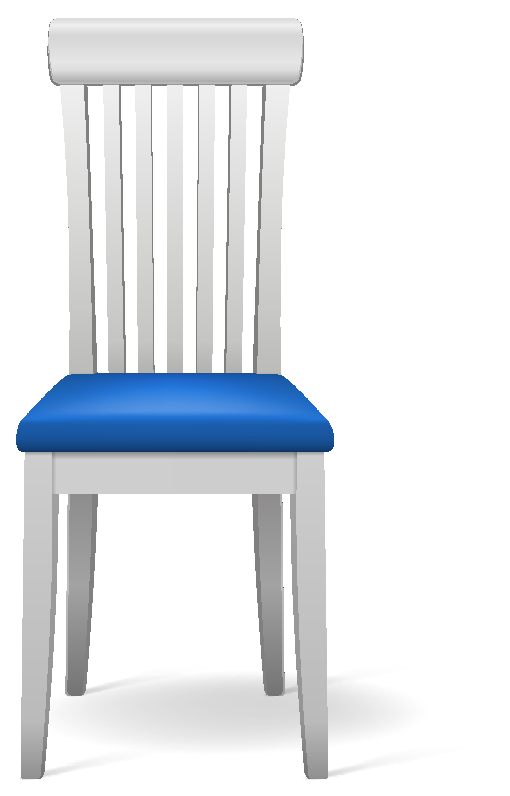
\includegraphics[height=1em]{chair/file.eps}}}$) \quad
  Tim Sherwood \quad
  Rich Wolski
}
\titlegraphic{\hfill
\includegraphics[width=2.25cm]{ucsbseal_cmyk.pdf}}

\begin{document}
\maketitle

\metroset{numbering=none}
\begin{frame}<beamer>[noframenumbering]
  \frametitle{Outline}
  \tableofcontents
\end{frame}
\metroset{numbering=fraction}

\section{Motivation}
\begin{frame}{What is a System?}
Infrastructure software upon which applications are built
\\
\vspace{0.2in}
\pause
Operating Systems % lowest level of abstraction
\todo{talk about applicability to other systems, like file systems}
  \begin{itemize}[<+->]
    \item Process abstraction
    \item Named resource management
       \begin{itemize}
           \item Multiplex physical hardware resources
           \item Partition and abstract \textbf{memory}
       \end{itemize}
    \item Low overhead, robustness, security
  \end{itemize}
\end{frame}

\note[itemize]{
  \item example: compilers, garbage collectors, file systems, drivers, etc.
  \item need to be able to do this
  \item isolation third item for os
  \item files: hide peculiarites of disks/I/O decives, abstract model of device-indepdent files
  \item address space: virtual memory + protection
  \item process: running program container (registers, files, alarms, address space, etc.)
}

\begin{frame}{Systems Languages}
\begin{itemize}[<+->]
    \item Past systems languages: \tiny{ALGOL, PL/I, Fortran, BCPL/B, C, Mesa/Cedar, Pascal/Modula-2/Oberon, C++, ...}
    \item C: the de-facto standard
        \begin{itemize}
            \item Data structure representation control \note{how it looks}
            \item Memory management control \note{where it is, how long it lives}
            \item Complete mutability via pointers \note{with systems without protected address space, can literally write anything; embedded have memory-mapped I/O}
            \item Performant
            \item Legacy \note{alas: have to deal with it}
        \end{itemize}
    \item C: the unsafe standard
        \begin{itemize}
            \item Unchecked array operations $\Rightarrow$ buffer overflows
            \item Pointers $\equiv$ arrays $\Rightarrow$ hazardous pointer arithmetic
            \item Unsafe casts $\Rightarrow$ read/write arbitrary addresses, untyped
            \item Aliasing $\Rightarrow$ dangling pointers, double frees, null dereferences
            \item Undefined behavior $\Rightarrow$ \todo{insert nuke}
        \end{itemize}
\end{itemize}
\end{frame}

\note[itemize]{
\item possibly add OS lang was used for, date
\item ALGOL: formally defined syntax (OS: Burroughs, VME, Cambridge CAP)
\item PL/I: (OS: Multics)
\item Mesa, Cedar: rich exceptions, GC
\item Pascal (1971), Modula-2 (1982), Oberon (1988)
\item -- structured programming
\item -- records
\item -- pointers,
\item -- dynamic allocation,
\item -- information hiding,
\item -- objects
% see mae3.org, mae4.org
}

\begin{frame}{Memory Safety}
\begin{itemize}[<+->]
    %\item Memory safety error: ``Any dereference of a pointer or subscripted array reference which reads or writes storage outside of the referent'' \footcite{austin_efficient_1994}
    \item Memory safety error: Dereferencing a pointer which reads or writes storage outside of the referent
        \begin{itemize}
            \item Spatial: outside referent's \alert{address bounds}
            \item Temporal: outside referent's \alert{lifetime}
        \end{itemize}
        % TODO add graphic showing what I mean by referent
    \item Ideal technique is
        \begin{itemize}
            \item Efficient and expressive % (hallmarks of C)
            \item Purely static % (no runtime overhead, we will not have if we want computer help)
            % note: checking buffer overflows is generally undecidable
            \item Precise % (not overly conservative)
            \item Automatic % (legacy code $\Rightarrow$ no source or memory layout change)
        \end{itemize}
%    \item Non-goals: secrecy, security, concurrency, type safety % but are natural consequences of safety
    \item Memory errors become \alert{type errors}, management happens at \alert{compile-time}
\end{itemize}
\end{frame}

\note[itemize]{
\item some of those goals from nagakatte 201*
\item undecidability of checking certain dynamic errors
\item hard to verify/prove invariants about b/c
\item -- casts + pointers make c essentially untyped (rondon: type system is only to help know size of bytes to read/write)
\item -- aliasing
\item make bad hard, useful easy
}

\AtBeginSection[]
{
  \metroset{numbering=none}
  \begin{frame}<beamer>[noframenumbering]
    \frametitle{Outline}
    \tableofcontents[currentsection]
  \end{frame}
  \metroset{numbering=fraction}
}

\AtBeginSubsection[]
{
  \metroset{numbering=none}
  \begin{frame}<beamer>[noframenumbering] 
    \frametitle{Outline}   
    \tableofcontents[currentsection,currentsubsection]
  \end{frame}
  \metroset{numbering=fraction}
}

\only<handout>{
  \addtocounter{framenumber}{1}
}

\section{Spatial Safety}

\begin{frame}{Spatial Safety}
Always access within object's \alert{bounds}
\\
\pause
\vspace{0.2in}
\todo{insert picture}
\\
Some approaches:
\begin{itemize}
      \item Fat Pointers and Shadow Structures
      \item Referent Objects
      \item Dependent Types
%      \item Hardware
  \end{itemize}
\end{frame}

\begin{frame}[fragile]{Spatial Safety Example}
\begin{columns}[T]
\begin{column}{0.52\textwidth}
\begin{lstlisting}[
    language=C,numbers=left,mathescape,basicstyle={\small\ttfamily},
    moredelim={**[is][{\btHL<1>}]{@1}{@}},
    moredelim={**[is][{\btHL<2>}]{@2}{@}},
    moredelim={**[is][{\btHL<3>}]{@3}{@}},
    moredelim={**[is][{\btHL<4>}]{@4}{@}},
    moredelim={**[is][{\btHL<5>}]{@5}{@}},
    moredelim={**[is][{\btHL<6>}]{@6}{@}},
    moredelim={**[is][{\btHL<7>}]{@7}{@}},
]
@2int find_token(int *data,@
@2               int *end,@
@2               int token)@
{
    @3int *p = data;@
    @4while (p < end) {@
    @5    if (*p == token) break;@
    @6    p++;@
    }
    @7return (*p == token);@
}
\end{lstlisting}
\end{column} 
\begin{column}{0.44\textwidth}

\onslide<8->
\footnotesize{
Potential pointer dereference problems:
  \begin{itemize}[<+->]
      \item Null
      \item Uninitialized
      \item Out-of-bounds \note{related: data might not be an array, unrelated}
      \item Manufactured \note{not shown here exactly}
  \end{itemize}
}
\end{column}
\end{columns}

\end{frame}

\subsection{Fat Pointers and Shadow Structures}

\begin{frame}{Fat Pointers}
  \footnotesize
Fat Pointers
\pause
\begin{itemize}[<+->]
 \item Added information such as base and bound addresses (multiword) \note{typically info next to pointer}
 \item Instrument all pointers and functions
 \item Insert runtime checks \alert{before dereferences}, not arithmetic \note{as opposed to during arith, let arithmetic happen as usual}
 \item Advantages:
     \begin{itemize}
        \item Quickly find and retrieve metadata \note{no costly db lookup}
        \item Complete spatial safety \note{only way to enforce complete spatial safety is tracking ptr bnds}
        \item No sub-object overflows \note{will explain next section}
     \end{itemize}
 \item Disadvantages:
     \begin{itemize}
        \item Breaks binary compatibility \note{calling convention of external/uninstrumented libraries, storing pointer in register, casting ptr to int and back}
        \item Metadata propagation on every pointer assignment
        \item Unsafe casts can overwrite metadata
        \item Bloated code size and memory usage \note{because of added checks, bigger ptrs}
        \item Runtime overhead (up to 200\%)
     \end{itemize}
\end{itemize}
\end{frame}
% write wrappers to remove inline metadata before calling outside function
% have to instrument malloc...

\note[itemize]{
\item Source-code annotations, for some
\item Impractical for large code bases
\item Two distinct pointers can point to same object and have diff base/bounds associated with them
\item Overcomes sub-object overflows b/c can be detected b/c uniqueness of each ptr
}

\begin{frame}{Memory Layout}
    \todo{show how pointers are expanded with metadata}
    %$\vcenter{\hbox{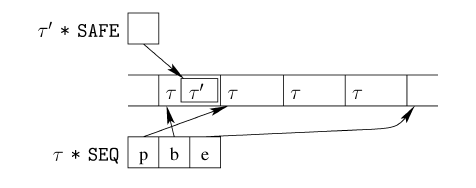
\includegraphics[height=6em]{fig/FIGURE_necula-2005_ccured-seq.PNG}}}$
\end{frame}

% possibly show example code of their fat pointers, or how memory changes, or...
\begin{frame}{Fat Pointer Approaches}
SafeC \footcite{austin_efficient_1994}:
\begin{itemize}
  \item \alert{Safe} pointers have value, base, and size
  \item Complete spatial safety, conditioned on \alert{transparent} storage management and no safe pointer attribute \alert{manipulation} \note{no domain-specific allocator at user-level}
  \item 275\% space overhead, 2-6x runtime overhead, 0.35-3x code size overhead \note{no register allocated safe ptrs, compiler optimizations fail with additional checks}
  \item Some static optimization based on still-valid previous checks
\end{itemize}
\vspace{0.1in}

%TODO {maybe "Low-cost concurrency checking of pointers" Patil 1997}
%TODO {maybe "Bounds-checking entire programs without recompiling" Nethercote 2004}

Cyclone \footcite{jim_cyclone:_2002}: \note{offshoot of TAL/popcorn}
\begin{itemize}
    \item Annotations for array/non-array pointers (never-null, fat, unitialized warning via control-flow analysis) % TODO look up again, split this
    \item Tagged unions and automatic tag injection (e.g. $\texttt{printf}$) %TODO remove or explain
    \item Can specify number of elements pointer points to \note{deputy is more general}
    %\item Arrays and strings converted automatically to fat
    % TODO determine if these are important
    %\item Statically validate and remove non-array fat pointers
    %\item 40\% runtime overhead
    %\item Uses regions + automatic memory management for temporal safety (free is a no-op) (see nice example)
    %\item never null don't need checks, use @; push back null checks from uses to their sources
    %\item ? permits pointer arithmetic
    %\item Restrict arithmetic on regular pointers
    %\item parametric polymorphism, subtyping, static analysis to check for safety, adding run-time checks
\end{itemize}
\end{frame}

\begin{frame}{Fat Pointer Approaches}
CCured \footcite{necula_ccured:_2002}:
\begin{itemize}
    \item \todo{how improves Cyclone?, check follow bullets/shrink}
    \item deep copies of ptrs when interacting with external libraries via wrppers
    \item Needs whole-program inference to detect pointers used unsafe type casts (WILD, can overwrite ptr info)
    \item reduce metadata propagation by using a type system to infer ptr usage: classify pointers as SAFE, SEQ, and WILD
    \item optimizes inserted checks and code for popagating metadata for each ptr kind
    \item \todo{show example judgement of how it knows to insert a runtime check, p5}
  % 'essentially union of two langs: strongly-typed lang (containing safe/seq pts), and untyped lang for which type infor is maintained and checked at runtime'
  % TODO does user have to annotate some??
  %\item Strong type system helps \alert{inference} statically \alert{optimize} different pointer uses % whole program type inference % TODO does previous attempts not do inference
  %    \begin{itemize}
  %        \item $\texttt{SAFE}$: almost no overhead, no: ptr. arith, array indexing, type casts % TODO are these never-null?
  %        \item $\texttt{SEQ}$: fat pointers, allow: arith, indexing, some casts
  %        \item $\texttt{WILD}$: arbitrary casts, expensive dynamic checks % All regular pointers are turned into this
  % WILD/DYNAMIC: ptr type does not carry wit it the type of values pointed to
  %      \end{itemize}
  %          \item Very detailed description of run-time checks generated and translation for each expression
  %          \item Relies on a garbage collector
  %\item 3\%-87\% runtime overhead increase
\end{itemize}
\vspace{0.1in}

% TODO add CCured 2002 judgment for command assertion insertion
% TODO acutally 2005 is better

Fail-Safe C \footcite{oiwa_implementation_2009}:
\begin{itemize}
    \item Combines fat pointers w/ fat integers and virtual structure offsets
\end{itemize}

\end{frame}

% use CCured syntax (2002, 2005 has a good translation definition)
\begin{frame}[fragile]{Fat Pointers Preventing Spatial Errors}
    \begin{columns}[T]
      \begin{column}{0.44\textwidth}
\begin{lstlisting}[language=C,numbers=left,mathescape,basicstyle={\scriptsize\ttfamily}]
int find_token(int *data,
               int *end,
               int token)
{
    int *p = data;
    while (p < end) {



        if (*p == token) break;


        p++;
    }

    return (*p == token);
}
\end{lstlisting}
\end{column}

\pause

\begin{column}{0.56\textwidth}

\begin{lstlisting}[language=C,numbers=left,mathescape,basicstyle={\scriptsize\ttfamily},
    moredelim={**[is][\btHL<3>]{@3}{@}},
    moredelim={**[is][{\btHL<4>}]{@4}{@}},
    moredelim={**[is][{\btHL<5>}]{@5}{@}},
    moredelim={**[is][{\btHL<6>}]{@6}{@}},
    moredelim={**[is][{\btHL<7>}]{@7}{@}},
    moredelim={**[is][{\btHL<8>}]{@8}{@}}
]
int find_token(int *@3SEQ@ data,
               int *@4SAFE@ end,
               int token)
{
    int *@5SEQ@ p = data;
    while (p < end) {
        @6assert(p.base != 0 &&@
        @6         0 <= p.value &&@
        @6         p.value < p.bound);@
        if (*p == token) break;
        @7p.value = p.value + (1 * sizeof(int));@
        @7p.base  = p.base;@   // optimized out
        @7p.bound = p.bound;@  // "           "
    }
    @6...(repeat lines 6-8)...@
    @8return (*p == token);@
}
\end{lstlisting}
\end{column}

\end{columns}
\end{frame}

\begin{frame}{Pointer-Based -- Shadow Structures}
Split metadata from pointer
\begin{itemize}
    \item Every value has linked shadow structure mirroring entire data structure
    \item Does not handle arbitrary casts % TODO why not, add info
    \item Out-of-sync metadata after external library code
    \item Generate metadata for library routines returning newly allocated object
\end{itemize}
\vspace{-0.1in}
CCured (2005) \footcite{necula_ccured:_2005} \note{improves original CCured work}
  \begin{itemize}
     \item Reduce number of WILD pointers
     \item Use physical subtyping \footcite{siff_coping_1999} for upcasts
     \item Special pointer carrying runtime type info for downcasts
  \end{itemize}
\vspace{-0.1in}
MSCC \footcite{xu_efficient_2004}
  \begin{itemize}
     \item Optimized encoding loses ability to detect sub-object overflows
  \end{itemize}
\end{frame}

% MSCC style
\begin{frame}[fragile]{Shadow Structures Example}
\begin{columns}
\begin{column}{0.42\textwidth}
\begin{lstlisting}[language=C,numbers=left,mathescape,basicstyle={\scriptsize\ttfamily}]




int find_token(
  int *data,
  int *end,
  int token)
{
    int *p = data;

    while (p < end) {

        if (*p == token) break;
        p++;
    }

    return (*p == token);
}
\end{lstlisting}
\end{column}

\pause

\begin{column}{0.56\textwidth}

\begin{lstlisting}[language=C,numbers=left,mathescape,basicstyle={\scriptsize\ttfamily},
    moredelim={**[is][{\btHL<3>}]{@3}{@}},
    moredelim={**[is][{\btHL<4>}]{@4}{@}},
    moredelim={**[is][{\btHL<5>}]{@5}{@}},
    moredelim={**[is][{\btHL<6>}]{@6}{@}},
]
@3struct ptr_info {@
@3    void *base;@
@3    unsigned long bound;@
@3};@
int find_token(
  int *data, @4ptr_info *data_info,@
  int *end,  @4ptr_info *end_info,@
  int token)
{
    int *p = data;
    @5ptr_info  p_info = *data_info;@
    while (p < end) {
        @6CHECK_SPATIAL(p, sizeof(*p), p_info);@
        if (*p == token) break;
        p++;
    }
    @6CHECK_SPATIAL(p, sizeof(*p), p_info);@
    return (*p == token);
}
\end{lstlisting}
    \end{column}
  \end{columns}
\end{frame}

% TODO question: where is table stored (heap or stack?)
% TODO insert table-of-contents

\subsection{Referent Objects}

\begin{frame}[fragile]{Referent Objects}
Objects
\footnotesize
\begin{columns}[T]
\begin{column}{0.45\textwidth}
\begin{itemize}[<+->]
    \item Associate metadata with \alert{objects} themselves, not pointers
    \item Global database relates every allocated address to corresponding object metadata \note{updating on alloc, dealloc, on function entry/exit for stack-based objects, program startup for global object}
    \item Every pointer to same object shares same metadata
    \item Bounds check on \alert{pointer arithmetic} \note{and array indexing} to ensure validity of derived poitners \note{i.e. point to same object}
    %\item do not check pointer derferences
\end{itemize}
\end{column}

\pause

\begin{column}{0.45\textwidth}
Advantages:
\begin{itemize}
  \item Compatible with uninstrumented code \note{no memory layout change; if pointer updated by untrusted module, metadata out-of-sync}
\end{itemize}
\pause
Disadvantages:
\begin{itemize}
  \item Special mechanisms to handle legal OOB pointers \note{since going 1 past array undereferenced is legal C}
  \item Splay-tree object lookup overhead
  \item Incomplete spatial safety: \alert{sub-object overflows} \note{type casts, mem corruption in objects, C allows ptr arith in struct fields}
\end{itemize}
\pause

\begin{lstlisting}[
    language=C,numbers=left,mathescape,basicstyle={\tiny\ttfamily},
    moredelim={**[is][{\btHL<1>}]{@1}{@}},
    moredelim={**[is][{\btHL<2>}]{@2}{@}},
    moredelim={**[is][{\btHL<3>}]{@3}{@}}
]
struct {char str[8]; void (*func)(); } node;
char *ptr = node.str
strcpy(ptr, "overflow...");
\end{lstlisting}
\end{column}
\end{columns}

\end{frame}

% TODO show in memory example of subobject problem

\note[itemize]{
\item Because nested objects (e.g., an array of structures) are assigned base and bound addresses
\item that span the entire allocated region, it is impossible to detect sub-object overflows if an
\item out-of-bounds pointer to an inner object remains within bounds of the outer object.
}

% TODO possibly "Applied to linux kernel: Criswell Secure virtual arch 2007"

\begin{frame}{Referent Objects Approaches}
J\&K \footcite{jones_backwards_1997}
    \begin{itemize}
       %\item Maintain table of all known valid storage objects
       %\item Map a ptr to a desciptor of the object into which it points
       \item Pad objects w/ extra byte \todo{why}
       %\item check ptr arith and use, b/c result cannot refer to diff object from one from which it is originally derived
       %\item object for which the ptr is valid is only determined by checking ptr itself, looking it up in object table
       \item Incomplete because cannot pad parameters \note{would change layout}
       \item 11-12x overhead
    \end{itemize}
\vspace{0.2in}

CRED \footcite{ruwase_practical_2004}
    \begin{itemize}
      \item More generic solution \todo{how}
      \item 2x overhead
    \end{itemize}
\vspace{0.2in}
\end{frame}

\begin{frame}[fragile]{Referent Objects Approaches}
SafeCode \footcite{dhurjati_2006_backwards}
    \begin{itemize}
        \item Use automatic pool allocation (APA) \footcite{lattner_automatic_2005} \note{builds on JK, APA: partitions memory based on static points-to analysis}
        \item Use separate, \alert{smaller} data structures to store bounds metadata for \alert{each partition}
        \item 1.2x overhead
    \end{itemize}
\vspace{0.2in}

Baggy Bounds Checking (BBC) \footcite{akritidis_baggy_2009}
    \begin{itemize}
    \item Trades memory for performance \note{fastest object bounds checker}
    \item Pads every object s.t. size is power of two, aligns base addresses to be multiple of their padded size
    \item Compact bounds representation, efficient way to look up object bounds
    \item 0.6x overhead \note{on SPECINT 2000 benchmark}
    \end{itemize}
\vspace{0.2in}
% TODO read this paper more: great succinct explanation of this approach (p 2)

%PariCheck \footcite{younan_paricheck_2010} \note{like BBC, faster/lower overhead}
\end{frame}

\begin{frame}[fragile]{Referent Objects Example}
\footnotesize
\begin{columns}[T]
\begin{column}{0.42\textwidth}
\begin{lstlisting}[language=C,numbers=left,mathescape,basicstyle={\scriptsize\ttfamily}]
int find_token(int *data,
               int *end,
               int token)
{
    int *p = data;
    while (p < end) {
        if (*p == token) break;




        p++;
    }
    return (*p == token);
}
\end{lstlisting}
\end{column}

\pause

\begin{column}{0.56\textwidth}
\begin{lstlisting}[
    language=C,numbers=left,mathescape,basicstyle={\scriptsize\ttfamily},
    moredelim={**[is][{\btHL<3>}]{@3}{@}},
    moredelim={**[is][{\btHL<4>}]{@4}{@}},
    moredelim={**[is][{\btHL<5>}]{@5}{@}},
    moredelim={**[is][{\btHL<6>}]{@6}{@}},
]
int find_token(int *data,
               int *end,
               int token)
{
    int *p = data;
    while (p < end) {
        if (*p == token) break;
        @3int *q = p + 1;@
        @4int size = 1 << TABLE[p>>SLOT_SIZE];@
        @5int base = p & ~(size - 1);@
        @6assert(q >= base && q - base < size);@
        p++;
    }
    return (*p == token);
}
\end{lstlisting}
%Lines 4-6 are equivalent to $\texttt{assert((p^q)>>TABLE[p>>SLOT_SIZE] == 0)}$.
\end{column}

\end{columns}
\end{frame}

% TODO add diagram of memory layout and how this ptr arith works!!!

% Mudflap: Eigler 2003
% Criswell: Secure Virt Arch 2007
% PariCheck: Younan: 2010


%\begin{frame}{Fat Pointers}
%\todo{put somewhere else}
%Cuckoo \footcite{west_cuckoo:_2005}
%      \begin{itemize}
%          \item Store array size in memory before array dimensions' first element
%          \item Name of an array is pointer to an \emph{array}, not first object
%          \item Type system for preventing assignment of automatic objects into longer-lifetime pointers
%          %\item Wrap dynamic memory allocation (type homogeneous pool-based) % will explain later
%          \item Forbid addition and subtraction expressions including pointer operands! % TODO what?! statically determining given pointer points to an array object is undecidable
%        % compile-time checks if array bounds are constants, otherwise run-time checks
%      \end{itemize}
%\end{frame}

\begin{frame}{Softbound}
\footnotesize
Softbound \footcite{nagarakatte_softbound:_2009}
    \begin{itemize}[<+->]
        \item Base and bound metadata for each pointer, stored in disjoint metadata space (via table lookups) \note{like pointer-based and object approaches, two-level trie data structure in disjoint metadata space}
        \item Total spatial safety of pointer-based approaches \note{eliminate sub-object problem}
        \item Source compatibility, separate compilation of object-based approaches
        \item Runtime bounds checks on each dereference
        \item Propagate metadata as extra arguments \note{to function calls, wrappers for commonly-used libraries, must transform every func decl/call-site, or shadow stack (nagarakatte thesis)}
        \item Arbitrary casts allowed \note{just check ptr involved in casts on derfernce w.r.t to its metadata, no way to overwrite metadata}
        \item 67\% overhead
%        \item Must protect every module for *complete* safety (untrusted module can modify ptr, table is out-of-sync)
%        \item Only store metadata in disjoint space for pointers in memory, perform metadata loads/stores only when loaded/stored value from/into memory loc is a ptr
%        \item Wrappers for commonly used libraries
    \end{itemize}
\end{frame}
% TODO lookup how 'lookup works'

\begin{frame}{Softbound Example}
    \todo{possibly}
\end{frame}

% TODO update running example, or add in softbounds pictures! (or reserve for CETS)

%\begin{frame}{Hardware Approaches to Spatial Safety}<presentation:0>
%    \begin{itemize}
%       \item Hardbound: Devietti 2008
%       \item Intel MPX %: \verbatim{https://gcc.gnu.org/wiki/Intel%20MPX%20support%20in%20the%20GCC%20compiler}
%       \item Watchdog: Nagarakatte 2012
%       \item (Hybrid): WatchdogLite
%    \end{itemize}
%\end{frame}

%\begin{frame}{Other Spatial Approaches}<presentation:0>
%\begin{itemize}
% \item (Also: tripwire approaches, mostly for testing): TODO need to have reason why I'm skipping
% \item Hastings Purify 1992 (reveal during testing), object based, has temporal safety
% \item Nethercote Valgrind 2007 (reveal during testing)
% \item Qin SafeMem 2005
% \item Venkataramani Memtracker 2007
% \item Yong "Protecting C" 2003
% \item Serebryany AddressSanitizer 2012: object-based, has temporal safety
%\end{itemize}
%\end{frame}

% TODO describe why not mentioning ETC/LCLint/CSSV/Abcd are static analyzers, not built-in lang techniques

\subsection{Dependent Types}

\begin{frame}{Dependent Types}
    Dependent types are \emph{typed-valued functions} \footcite{pierce_advanced_2005}
    % type family of vectors
    % dependent product type
\begin{center}
   $\texttt{Vector : Nat}\rightarrow\texttt{*}$
   $\texttt{vecnew : }\Pi\texttt{n:Nat.data}\rightarrow\texttt{Vector n}$
   $\texttt{cons : }\Pi\texttt{n:Nat.data}\rightarrow\texttt{Vector n}\rightarrow\texttt{Vector(n+1)}$
\end{center}

    \begin{itemize}
        \item Based on type theory work by Martin-L\:of \footcite{martin-lof_constructive_1984}
        \item Undecidability of type checking: arbitrary computation/proof to establish equality of two types
        \item Various of following approaches work on definining equality and restricting forms of index terms
    \end{itemize}
\end{frame}

\begin{frame}{Dependent Types in Functional Languages}
\vspace{-0.08in}
Dependent ML (DML) \footcite{xi_eliminating_1998}
\begin{itemize}
    \item Reduce static array bound checking to constraint satisfiability
    \item Indexed types: limit indices to linear integer and boolean expressions; compile-time decidable \note{decidable logic}
    \item User provides types of recursive procedures and inductive datatypes
\end{itemize}
Cayenne (Haskell-like) \footcite{augustsson_cayennelanguage_1998}
\begin{itemize}
    %\item First time \emph{full dependent} types in a PL % TODO say
    \item No restriction on expressions in types
    %\item Example typing a C-style $\texttt{printf}$ function where $\texttt{PrinftType}$ returns a type % TODO say
    \item Undecidability of arbitrary expression equivalence and thus type checking
\end{itemize}
$\text{Xanadu}_{0}^{\Pi,\Sigma}$ (C-like) \footcite{xi_imperative_2000}
\begin{itemize}
    \item Like DML, restrict index expressions in types to integer constraint domain
%    \item Defines what it means for a type to equal/coerce into another
    \item Programmer must supply state type in order to type conditionals and loops \todo{remove?}
\end{itemize}
    \vspace{0.2in}
\end{frame}
\note[itemize] {
\item the goal here is just to show that FuncLangs did it first, but they aren't always practical b/c of undecidability, difficult to use
\item infuttered form, you get CoC
}

% \item Allows trusted cast mechanism to supress errors

\begin{frame}{Dependent Types in Imperative Languages}
SafeDrive \footcite{zhou_safedrive:_2006} and Deputy \footcite{condit_dependent_2007}, \footcite{anderson_static_2007}
%\vspace{-0.1in}
    \begin{itemize}[<+->]
        \item User-added annotations relating pointers to bounds
            \begin{itemize}
                \item \texttt{safe}, \texttt{sentinel}, \texttt{count(n)}, \texttt{bound(lo,hi)}
                \item Use constants/variables/field names in immediately enclosing scope \note{n, lo, hi are expressions}
            \end{itemize}
        %\item allow programmers to specify common c programming idioms involving ptr arith and union types
        %\item compiler checks safety of most pointer and union operations
        \item Three-phase pass over annotated C programs, emits C code
            \begin{enumerate}
                \item Automatic addition of bounds annotations for pointer types \note{fresh local var to hold bounds}
                \item Flow-insensitive type checking (insert run-time checks, helps decidability) \note {hybrid means SA for type determination, run-time checks when SA precision is too low}
                \item Flow-sensitive check optimization
            \end{enumerate}
        \item More C Support: mutable structures, dependent union tags \note{c idiom: tag indicates union field in use}, Safe TinyOS \footcite{hill_system_2000}, \footcite{gay_nesc_2003}, \footcite{cooprider_efficient_2007}
    \end{itemize}
    \vspace{0.2in}
\end{frame}

\note[itemize]{
% they're really *hybrid* approach: try your best, then offer runtime checks
% TODO maybe include this info (next few items)
  \item track info required to place run-time checks (asserts) in program
  \item  flow- path-insensitive, bolvious to aliasing, heap updates, data structures
  \item local type inference
  \item static verifier discharges checks at compile-time
% about annotations
  \item safe = ptr is null/pts to single element of base type
  \item sentintel = only for comparisons
  \item count(n) = null or point to an array of at least nelements of base type
  \item bounds(lo,hi) = null or point into mem region w/ low address lo, hi is first element beyond region end
  \item: invariant is that ptrs null, or within stated bounds
% dependent union tags
  \item c idiom: tag indicates union field in use
  \item Specify the condition for each union field to be usable
  \item \emph{$\text{union}_n\ \tau_1\ ...\ \tau_n\ e_1\ ...\ e_n$}
  \item $x:\text{struct }\{ tag:\text{int}\;\ u: \text{union}_2 \text{ int (ref int)} \ (\textit{tag} \geq 2)\ (\textit{tag} = 1) \}$
% generalized ptr
  \item Generalize array constructor to possibly-null bounded pointer
  \item C-style pointer arithmetic via $\oplus$ operator % TODO why use that special symbol?
  \item $x:\text{ptr int } x\ (x \oplus n)$ $\texttt{// n integer area starting at x}$
  \item $x:\text{ptr int } x\ e\ \ \ \ \ \ \ \ $ $\texttt{// from x to e}$
% TODO: are the assertions to make it safe (catch bad things), or an assertion something that is known to be true
}

% go through an example to get a feeling, then after explaining judgments, explain it again stepping through the judgments
\begin{frame}[fragile]{Deputy Example for Spatial Safety}
\begin{columns}[T]
\begin{column}{0.40\textwidth}
\begin{lstlisting}[language=C,numbers=left,mathescape,basicstyle={\scriptsize\ttfamily}]
int find_token(int *data,
               int *end,
               int token)
{


    int *p = data;
    while (p < end) {


        if (*p == token) break;

        p++;
    }


    return (*p == token);
}
\end{lstlisting}
\end{column}

%\scriptsize{$\colorbox{blue!30}{Code added during automatic dependency inference}$}

\pause

\begin{column}{0.58\textwidth}
\begin{lstlisting}[
    language=C,numbers=left,mathescape,basicstyle={\scriptsize\ttfamily},
    moredelim={**[is][{\btHL[onslide=<3->{fill=blue!50}]}]{@3}{@}},
    moredelim={**[is][{\btHL[onslide=<4->{fill=blue!50}]}]{@4}{@}},
    moredelim={**[is][{\btHL[onslide=<5->{fill=blue!50}]}]{@5}{@}},
    moredelim={**[is][{\btHL[onslide=<6->{fill=red!50}]}]{@6}{@}},
    moredelim={**[is][{\btHL[onslide=<7->{fill=red!50}]}]{@7}{@}},
    moredelim={**[is][{\btHL[onslide=<8->{fill=red!50}]}]{@8}{@}},
    moredelim={**[is][{\btHL[onslide=<9->{fill=red!50}]}]{@9}{@}},
]
int find_token(int * @3bound(cur, end)@ data,
               int * @4sentinel@ end,
               int token)
{
    @6assert(data != NULL);@
    @6assert(end != NULL);@
    int *p @5bound(cur, end)@ = data;
    while (p < end) {
        @7assert(p != NULL);@
        @7assert(p < end);@
        if (*p == token) break;
        @8assert(p <= p + 1 <= end);@
        p++;
    }
    @9assert(p != NULL);@
    @9assert(p < end);@
    return (*p == token);
}
\end{lstlisting}
\end{column}
\note[itemize]{
\item Let's assume that the code is fully annotated (automatic generation coming later)
\item No arithmetic/comparisons on null ptrs
\item 8 assert: legal to point past end
\item 9 illegal to access
}

\end{columns}
\end{frame}
% \note{All checks here would be eliminated}

% \note{here I need to exaplin what a grammer is for them}
\begin{frame}{Abstract Syntax, For Your Consideration}
\begin{gather*}
    x,y \in \text{Variables}
    \quad
    \text{op} \in \text{Binary ops}
    \quad
    n \in \text{Integers}
    \quad
    \text{comp} \in \text{Comparison Ops}
\end{gather*}

\vspace{0.2in}

\begin{columns}[T]
\begin{column}{0.45\textwidth}
\begin{alignat*}{2}
\text{Ctors}\quad &C &&::= \text{int} \altm \text{ref} \altm ...
\\
\text{Types}\quad &\tau &&::= C \altm \tau_1 \ \tau_2 \altm \colorIt{blue}{n1}{\tau\ e}
\\
\text{Kinds}\quad & \kappa &&::= \text{type} \altm \text{type} \rightarrow \kappa \altm \tau \rightarrow \kappa
\\
\text{L-exprs} \quad &l &&::= x \altm *e
\end{alignat*}
\end{column}

\begin{column}{0.45\textwidth}
\begin{alignat*}{2}
\textit{Exprs}\quad &e &&::= n \altm l \altm e_1 \text{ op } e_2
\\
\textit{Cmds}\quad &c &&::= \text{skip} \altm c_1;c_2 \altm l := e \altm \colorIt{red}{n2}{\text{assert}(\gamma)} \altm
\\
~ & ~ && \text{let } x : \tau = e \text { in } c \altm \text{let } x = \text{new } \tau(e) \text{ in } c
\\
\colorIt{green}{n3}{\text{Preds}} \quad &\gamma &&::= e_1 \text{ comp } e_2 \altm \text{true} \altm \gamma_1 \wedge \gamma_2
\end{alignat*}
\end{column}
\end{columns}

\vspace{0.1in}
\end{frame}

%\scriptsize{$\colorbox{green!30}{Programmer-supplied annotation}$}

\note[itemize]{
\item kind of int is "type"
\item kind of ref is "type -> type"
\item loops, conditionals omitted for flow-insenstivei type system
\item Types restricted to only contain expressions using constatns, local variables, arbitrary arithmetic operators
\item Type environment is a predicate on the state of the program
}

% todo add some color, at least to one or two judgments for explanation
\begin{frame}{Typing Rules, For Your Consideration}
Deputy judgments and type checking rules:
\note{local expression: expressions formed using constants, local variables, arbitrary arithmetic operators (no memory deferences}
\note{expressions in types are restricted to local expressions}
% TODO color these based on the type of judgement (in line above this one and in judgment name)
% TODO make an animation

\pause

Local Expressions
\begin{center}
\begin{tabular}{cc}
\infer[(\textsc{local\ name})]
{\Gamma \vdash_{L} x : \tau }
{\Gamma(x) = \tau}
    &
\infer[(\textsc{local\ num})]
{\Gamma \vdash_{L} n : int }
    {}
\end{tabular}
\end{center}

\pause

Non-local Expressions
\begin{center}
\begin{tabular}{c}
\infer[(\textsc{deref})]
{\Gamma \vdash *e : \tau \Rightarrow \gamma}
{\Gamma \vdash e: \text{ref } \tau \Rightarrow \gamma}
\end{tabular}
\end{center}

\pause

Commands
\begin{center}
\begin{tabular}{c}
\infer[(\textsc{var\ write})]
{\Gamma \vdash x \coloneqq e \Rightarrow \text{assert}(\bigwedge_{y \in \text{Dom}(\Gamma)}\gamma_y);\ x \coloneqq e }
{x \in \text{Dom}(\Gamma) \qquad
 \text{for\ all}(y:\tau_y) \in \Gamma,\ \Gamma \vdash y[e/x]:\tau_y[e/x] \Rightarrow \gamma_y }
\end{tabular}
\end{center}

\pause
\end{frame}

\begin{frame}{The Interesting Rules}
Dereferencing
\begin{center}
\begin{tabular}{c}
\infer[(\textsc{array\ deref})]
{\Gamma \vdash *e; \tau \Rightarrow \gamma_e \wedge (0 < e_{len})}
{\Gamma \vdash e: \text{array } \tau \ e_{len} \Rightarrow \gamma_e}
\end{tabular}
\end{center}

\vspace{0.1in}
\pause

Arithmetic
\begin{center}
\begin{tabular}{c}
\infer[(\textsc{array\ arith})]
{\Gamma \vdash e + e': \text{array } \tau\ (e_{len} - e') \Rightarrow \gamma_e \wedge \gamma_e' \wedge (0 \leq e' \leq e_{len})}
    {\Gamma \vdash e: \text{array } \tau\ e_{len} \Rightarrow \gamma_e
    \quad \Gamma \vdash e':\text{int} \Rightarrow \gamma_{e'}}
\end{tabular} 
\end{center}

\end{frame}
% var-write is a key contribution of type system
% $\textsc{var\ write}$ rule responsible for updates to variables in presence of dependent type variables, verifying assignment does not break any dependencies in current scope
% For example, we can add rules for arrays:
% also permits a coercion judgement for allowing an array to be used where a smaller one is expected
% todo how are constraints solved during phase 3?

% todo if time
%\begin{frame}[fragile]{Revisiting that Deputy Example}
%\begin{columns}[T]
%\begin{column}{0.45\textwidth}
%\begin{lstlisting}[
%    language=C,numbers=left,mathescape,basicstyle={\scriptsize\ttfamily},
%    moredelim={**[is][{\btHL[onslide=<3->{fill=blue!50}]}]{@3}{@}},
%    moredelim={**[is][{\btHL[onslide=<4->{fill=blue!50}]}]{@4}{@}},
%    moredelim={**[is][{\btHL[onslide=<5->{fill=blue!50}]}]{@5}{@}},
%    moredelim={**[is][{\btHL[onslide=<6->{fill=red!50}]}]{@6}{@}},
%    moredelim={**[is][{\btHL[onslide=<7->{fill=red!50}]}]{@7}{@}},
%    moredelim={**[is][{\btHL[onslide=<8->{fill=red!50}]}]{@8}{@}},
%    moredelim={**[is][{\btHL[onslide=<9->{fill=red!50}]}]{@9}{@}},
%]
%int find_token(int * @3bound(cur, end)@ data,
%               int * @4sentinel@ end,
%               int token)
%{
%    @6assert(data != NULL);@
%    @6assert(end != NULL);@
%    int *p @5bound(cur, end)@ = data;
%    while (p < end) {
%        @7assert(p != NULL);@
%        @7assert(p < end);@
%        if (*p == token) break;
%        @8assert(p <= p + 1 <= end);@
%        p++;
%    }
%    @9assert(p != NULL);@
%    @9assert(p < end);@
%    return (*p == token);
%}
%\end{lstlisting}
%\end{column}
%
%\pause
%
%\begin{column}{0.45\textwidth}
%    \todo{add explanation of use of rules}
%\end{column}
%
%\end{columns}
%\end{frame}


% TODO possibly reduce, mention in passing
\begin{frame}{Dependent Types in Imperative Languages}
% TODO revisit Low-Level Liquid Types, understand better!
Low-Level Liquid Types (LTLL) \footcite{rondon_liquid_2008}, \footcite{rondon_low-level_2010}
\begin{itemize}
    \item Refinement types where predicates are conjunctions over qualifiers
    \item Functions qualified over locations they operate on
    \item Deal with collections using \emph{location folding} for checking out a copy to do strong updates on
%    \item Tries to deal with lack of types, mutation, unbounded collections that make type-based mechanisms difficult
\end{itemize}
% TODO how is Tyr different/better than Deputy? its 2016, what changed?
T\'yr \footcite{de_araujo_tyr:_2016}
\begin{itemize}
    \item Augments LLVM IR with dependent pointer types
    \item Uses programmer annotations insert run-time bounds checks
    \item LLVM optimizations remove always-true checks; error if always-false
\end{itemize}
\vspace{0.2in}
\end{frame}

\begin{frame}{Checked C} % restricted form of dependent types
Checked C \footcite{ruef_checked_2017}
    \begin{itemize}
%        \item Focus on interoperablity, usability, performance
%        \item Discovers safely-used ptrs, rewriting them to be checked
%        \item Normal C pointers
        \item associated bounds expressions with each $\_Array\_ptr<T>$ type to indicate where bounds are stored
        \item Extend C with two \emph{checked pointer types} \note{automatically rewrite code to use when possible}
            \begin{itemize}
                \item foo
            \end{itemize}
        \item Derefence-only (no arith.) pointer, arithmetic-supporting (possibly null-terminated) pointer with bounds in type
%        \item $\verb{_Ptr<T>}$, a pointer for dereference only (no arith)
%        \item $\verb{_Array_ptr<T>}$ and $\verb{_Nt_array_ptr<T>_}$, supporting arith w/ bounds declarations in type (latter is null-terminated)
        \item Isolate (un)safe code with \emph{checked code regions} at file/func/block level; prevent unchecked pointer usage and certain casts
        \item Cannot blame checked code for violation
%       \item Compiler confirms restrictions maintained, inserts checks on ptr access
    \end{itemize}
\end{frame}

\begin{frame}{A Hybrid Approach}
Low* \footcite{protzenko_verified_2017}
\begin{itemize}
    \item DSL for verified, efficient low-level programming in F* %(ML-like language with dependent types)
    \item Goal: write efficient \& verified C in a high-level language
    \item Write F* syntax against library modelling lower-level view of C memory
    \item Model arrays by implementation abstract buffer type using references by hyper-stacks % TODO define hyperstacks, what do I mean here?
    \item Translate Low* to CompCert Clight
\end{itemize}
\end{frame}

\begin{frame}{Quick Spatial Recap}
Spatial Safety
\begin{itemize}[<+->]
    \item Arrays and pointers \note{Unsafe languages like C conflate arrays and pointers, casts eliminate any semblance of type guarantees, types are just for size}
    \item Undecidable \note{Completely detecting buffer overflow in general is undecidable, so we try runtime things}
    \item Fat pointers \note{complete spatial safety at cost of compatibility}
    \item Referent objects \note{partial safety and better compatibility}
    \item Dependent types \note{prove in-bounds access at compile-time, emit run-time checks for full safety}
%    \item Solution% seems to be
%        \begin{itemize}
%            \item Restrict C
%            \item Limited form of bounds type information
%            \item Constraint solving
%            \item Runtime checks
%        \end{itemize}
\end{itemize}
\end{frame}

\section{Temporal Safety}

\begin{frame}[fragile]{Temporal Safety}
Prevent accessing object that has been \emph{previously deallocated}
\\
\begin{itemize}
   \item Capability store
   \item Effects and regions
   \item Linear types, ownership, and borrowing
\end{itemize}
\end{frame}

% todo
\begin{frame}[fragile]{Temporal Safety Example}
\footnotesize
\todo{add new code for temporal example}
\begin{lstlisting}[
    language=C,numbers=left,mathescape,basicstyle={\small\ttfamily},
    moredelim={**[is][{\btHL<1>}]{@1}{@}},
    moredelim={**[is][{\btHL<2>}]{@2}{@}},
    moredelim={**[is][{\btHL<3>}]{@3}{@}},
    moredelim={**[is][{\btHL<4>}]{@4}{@}},
    moredelim={**[is][{\btHL<5>}]{@5}{@}},
    moredelim={**[is][{\btHL<6>}]{@6}{@}},
]
@2int find_token(int *data, int count, int token)@
{
    @3int i = 0;@
    @3int *p = data;@
    @4while ((i < count) && (*p != token)) {@
    @5    p++;@
    @5    i++;@
    }
    @6return (*p == token);@
}
\end{lstlisting}

\onslide<7->
\footnotesize{
Potential pointer dereference problems:
  \begin{itemize}
      \item Dangling pointers/memory leaks
      \item Double frees
  \end{itemize}

Really boils down to:
\begin{itemize}
    \item Preventing use-after-free
    \item Eliminating free entirely \note{so 'use-after' has no meaning}
\end{itemize}
}
\end{frame}

\begin{frame}{A Comment on Garbage Collection}
Garbage collection
    \begin{itemize}
        \item Relinquish control of object location and layout to runtime \note{disallow free}
        \item Non-zero overhead, sub-par memory use (drag) \note{time between unreachable and reclaimed}
        \item Complete temporal safety
        \item Used by several of the spatial approaches previously listed (e.g. Fail-Safe C, CCured etc. uses Boehm-Demers-Weister \footcite{boehm_garbage_1988})
        \item Others like Cling \footcite{akritidis_cling:_???} rely on a special allocators % TODO
            \note{Replace malloc: address space re-use only among objects of same type and alignment (type-safe memory re-use)}
    \end{itemize}
\end{frame}
% \footcite{austin_efficient_1994}
% \footcite{jones_backwards-compatible_1997}
% \footcite{xu_efficient_2004}

\subsection{Capability Store}

\begin{frame}
Several of the pointer- and object-based approaches in the previous section also exhibit complete temporal safety
    \begin{itemize}
        \item SafeC, MSCC, Patil 1997, Yong 2003
            \begin{itemize}
              \item capability store to record temporal capability of objects as they are created and destroyed
              \item additional temporal data created/propagated with s[atial metadata links to a ptr fo the temporal cap of its referent
            \end{itemize}
        \item CCured, FailSafeC
           \begin{itemize}
                \item use BDW conservative GC, replace calls to malloc, ignore free
                \item heapify local variables (prevent dangling ptrs to stack objects) so they are managed by GC
                \item GC negates C's predictability, avoids real-time guarantees, increases address space reqs, reduces reference locality, increases page fault/cache miss rates
            \end{itemize}
        \item CETS+Softbound (some spatial checks in sb help get complete temporal in cets), Memsafe
        \item \todo{add a few lines here}
    \end{itemize}
\end{frame}
% (Zorn: measured cost of conservative GC: 1993)
% TODO where to put these
% Pointer-based
%    * [ ] CETS: Nagarakatte 2010, SoftboundCETS: nagarakatte 2015
%    * [/] MemSafe: Simpson 2013
%    * [ ] Lee "Preventing use-after-free with dangling ptrs" 2015

\subsection{Effects and Regions}

\begin{frame}{The Question}
Can we get the \alert{compiler} to do the memory deallocation for us? % will require a restriction of paradigms/cooperation by the programmer
\\
Can we statically determine the lifetimes/last-uses of all values and remove them? \note{like automatic variables put on/popped off stack}
\end{frame}

% let's begin with effects and regions

\begin{frame}{Effects}
    Effect types describe the \emph{effects} of the computation leading to a value \footcite{pierce_advanced_2005}
    \\
    \todo{show how to briefly annotate our example}
\end{frame}

\begin{frame}{Effects}
    Fluent Languages \footcite{gifford_integrating_1986}, MFX \footcite{lucassen_polymorphic_1988}
  \begin{columns}[T]
    \begin{column}{0.68\textwidth}
        \begin{itemize}[<+->]
            \item Mix functional and imperative languages \note{determine which can be parallelized}
            \item Every expression has a \emph{effect class}, restricting which subroutines or sublanguage features it may use
            \item Identify memoizable (referrentially transparent) expressions via a side effect lattice % for concurrency
        \end{itemize}
    \end{column}

    \pause

    \begin{column}{0.30\textwidth}
    \vspace{-0.2in}
    \footnotesize{
    \begin{tikzpicture}
        \node (WRA) at (0,3) {$\{W\ (R)\ (A)\}$};
        \node (RA)  at (0,2) {$\{R\ (A)\}$};
        \node (A)   at (0,1) {$\{A\}$};
        \node (e)   at (0,0) {$\{\}$};
        \node[draw] at (2,3) {$\text{Procedure}$};
        \node[draw] at (1.95,2) {$\text{Observer}$};
        \node[draw] at (1.95,1) {$\text{Function}$};
        \node[draw, right= of e] {$\text{Pure}$};
      \draw (e) -- (A) -- (RA) -- (WRA);
    \end{tikzpicture}

    \vspace{0.1in}
    \pause
    E.g.
    \begin{itemize}
        \item \texttt{update} is Procedure
        \item \texttt{nth} is Observer
        \item \texttt{arrayCreate} is Function
        \item \texttt{length} is Pure
    \end{itemize}
    }
    \end{column}
  \end{columns}
  \vspace{-0.3in}
\end{frame}
\note[itemize]{
% fluent
\item observer: not cause side-effects; cannot perform assignments or call procedure
\item function: not cause side-effcts, value is not affected by side-effects; no assignments, cannot call up, cannot access update-able variables
\item pure: referentially transparent: does not cause side-ffects, value not affected by side-effects, returns same value each time evaluated
\item pure:  no asignments, no accessing updating variables, cannot allocate updateable variables
\item cannot call UP the lattice
% MFX:
\item show soundness of effect type system for FX language
\item use effect information to constraint parallel evaluation of expressions
\item effect-masking: side-effects taht cannot be observed outside of the given expression
\item show how type and effect info can be used to implement certain kinds of side-effect analyses
\item language extends work with:
\item effect classes
\item full abstraction over effects
\item unmaskable side-effects
\item soundness proof
}

\begin{frame}{Effects}
    Type and Effect Systems \footcite{nielson_type_1999}
    \begin{itemize}[<+->]
        \item Extend the simply-typed lambda calculus with annotations
        \item Various forms of analyses, incl. Side Effect Analysis and \alert{Region} Inference
    \end{itemize}

    \pause

%\begin{gather*}
%    x \in \text{Variables}
%    \quad
%    c \in \text{Constants}
%\end{gather*}

\vspace{-0.2in}
\begin{alignat*}{2}
    \text{Exprs}\quad &e &&::= c \altm x \altm \texttt{fn}_{\pi}\ x\ \Rightarrow e_0 \altm e_1\ e_2 \onslide<5->{\altm \texttt{new}_{\pi}\ x\ :=\ e_1\ \texttt{in}\ e_2} \onslide<6->{\altm!x} \onslide<7->{\altm x := e_0}
\\
    \text{Types}\quad &\tau &&::= \texttt{int} \altm \texttt{bool} \only<4-8>{\altm \tau_1 \rightarrow \tau_2} \only<9->{\altm \tau_1 \xrightarrow[]{\phi} \tau_2} \only<8>{\altm \tau\ \texttt{ref}} \only<9->{\altm \tau\ \texttt{ref}\ \varrho}
\onslide<10->{\\ \only<10-11>{\text{Effect}}\only<12->{\colorIt{blue}{n1}{\text{Region}}}\quad &\phi &&::= \{!\pi\} \altm \{\pi:=\} \altm \{\texttt{new}\ \pi\} \altm \phi_1 \cup \phi_2 \altm \emptyset}
\onslide<11->{\\ \text{PrgPts}\quad &\varrho &&::= \{\pi\} \altm \varrho_1 \cup \varrho_2 \altm \emptyset}
\end{alignat*}

\onslide<13->{
\begin{center}
    $\Gamma \vdash e\ :\ \tau \ \&\ \phi$
\end{center}
}

\vspace{0.1in}
\end{frame}
\note[itemize]{
\item region inference: compile-time determination of when to allocate regions, in which to allocate data
\item Ref. variable represented by set of points where it could have been created (\alert{region})
\item Annotate functions with actions they take (access, assignment, creation)
\item we call \pi the creation point
\item \tau ref \varrho is type of loc created at one of the program points in region \varrho
}

% BitC \footcite{shapiro_origins_2008} % a retrospective on BitC, what they were looking for (not too interesting)

\begin{frame}{Region-Based Memory Managememt}
    Regions \footcite{tofte_region-based_1997}
    \begin{itemize}[<+->]
        \item Divide heap into collection of sub-heaps (``regions'') \note{unbounded subheaps}
        \item Grows on individual allocation; \alert{entire} region deallocated \note{no individual object deallocation}
        \item Explicit region polymorphism \note{regions can be given as arguments to functions at runtime}
        \item Sound type system \alert{guarantees safety} of deallocations \note{both alloc and dealloc are explicit}
        \item Region inference identifies:
            \begin{itemize}
                \item Points where entire regions are allocated and deallocated
                \item Into which region values should go
            \end{itemize}
        \item Used in ML Kit
        \item Unreasonable object lifetimes b/c LIFO ordering of region lifetimes %(lifetime of expression must coincide with time takes to execute some subexpression)
    \end{itemize}
    \vspace{0.1in}
\end{frame}

\begin{frame}{Early Use of Regions}
    \footnotesize{
Capability Calculus \footcite{crary_typed_1999}
    \begin{itemize}
        \item Add aliasing info to capabilities; track copies to know when truly revoked
        \item Arbitrarily-ordered region allocation/deallocation
    \end{itemize}
\pause
RC \footcite{gay_language_2001}
    \vspace{-0.1in}
   \begin{itemize}
     \item Region-support for C, focus on preventing dangling pointers % aliasing!
     \item For each region, maintain a reference count of external pointers pointing to objects in region % deleteregion fails if count is zero
     %\item Type system + annotations ($\texttt{sameregion}, \texttt{traditional}, \texttt{parentptr}$) to help compiler remove annotation operations % no updating associated region % enforced by runtime checks
     %\item Annotations ($\texttt{sameregion}, \texttt{traditional}, \texttt{parentptr}$) to prevent updating associated region % enforced by runtime checks
     %\item Restrict C by disallowing arbitrary integer-to-pointer casts
     %\item Break cyclic data structures before deleting regions
     \item \alert{No} memory safety guarantee
% \item 27%-11% overhead
   \end{itemize}
\pause
Reaps \footcite{berger_reconsidering_2002}
    \vspace{-0.1in}
   \begin{itemize}
     \item Combine regions and heaps into ``reaps''
     \item Behave like regions until $\texttt{reapFree}$ deallocates individual object
     \item Place freed object on a heap; subsequent allocations use heap until exhausted
%     \item Use Lea allocator generally, unless you need fast regions (i.e. reaps) % what their study found
   \end{itemize}
}
    \vspace{0.2in}
\end{frame}

\begin{frame}{Regions in Cyclone}
    Cyclone\footcite{grossman_region-based_2002}, again!
    \begin{itemize}[<+->]
        % TODO review what i mean by lexically-scoped: i.e. region x { int i<x> = 5; ... }
        \item Three region types: single \alert{heap} region (lives forever), \alert{stack} regions (local-declaration blocks), \alert{dynamic} regions (lexically-scoped lifetimes)
        \item Region-polymorphic functions
        \item Annotate pointers with regions into which they point; must be live for dereference
        \item Lifetime subtyping: region A <: region B $\Leftrightarrow$ region A \alert{outlives} region B
        \item Can specify partial orders on region lifetimes between pointers
        \item Sane defaults: infer region annotations on pointer types  % intraprocedural analysis => need function prototypes
    \end{itemize}
    \vspace{0.1in}
\end{frame}

\begin{frame}[fragile]{Regions in Cyclone}
\footnotesize

  \begin{columns}[T]
    \begin{column}{0.50\textwidth}
      \begin{itemize}[<+->]
        \item Pointer can escape scope of their regions \note{via closures/existential types}
        \item Type system tracks \alert{capability} (set of live regions) on pointer dereference % no closures, but existential types can hide pointers to escape scope of their regions
        \item A function's \alert{effect} is the set of regions it might access
        \item Calculate function's effect from prototype alone
        \item Type of elements not known, so use $\epsilon$ to abstract set of regions it might need to access
        \item Fix with static operator $\texttt{regions\_of}$ instead of effect variables % TODO review what effect variables are
      \end{itemize}
    \end{column}

    \pause

\begin{column}{0.48\textwidth}

\begin{lstlisting}[language=C,numbers=left,mathescape,basicstyle={\footnotesize\ttfamily}]
struct Set<$\alpha$, $\rho$, $\epsilon$>
{
    list_t<$\alpha$, $\rho$> elts;
    int (*cmp)($\alpha$, $\alpha$; $\epsilon$);
}
\end{lstlisting}

\pause

\begin{lstlisting}[
    language=C,numbers=left,mathescape,basicstyle={\small\ttfamily},
    moredelim={**[is][{\btHL<8>}]{@8}{@}},
]
struct Set<$\alpha$, $\rho$>
{
    list_t<$\alpha$, $\rho$> elts;
    int (*cmp)($\alpha$, $\alpha$; @8regions_of}($\alpha$)@);
}
\end{lstlisting}

\end{column}
\end{columns}

\end{frame}

% TODO make an animation with colors describing things I talk about as I do
\begin{frame}{Some Cyclone Abstract Syntax}
\scriptsize{
\begin{alignat*}{2}
\text{kinds}\quad &\kappa &&::= T \altm R
\\
\text{type and region vars}\quad &\alpha,\rho &&
\\
\text{region sets}\quad &\epsilon &&::= \alpha_1 \cup ... \cup \alpha_n \cup \{\rho_1,...,\rho_m\}
\\
\text{region constraints} \quad &\gamma &&::= \emptyset \altm \gamma, \epsilon <: \rho
\\
\text{constructors} \quad &\tau &&::= \alpha \altm \text{int} \altm \tau_1 \xrightarrow[]{\epsilon} \tau_2 \altm \tau_1 \times \tau_2 \altm \tau \ast \rho \altm
\\
~ & ~ && \qquad \text{handle}(\rho) \altm \forall\alpha:\kappa \triangleright \gamma.\tau \altm \exists \alpha:\kappa \triangleright \gamma.\tau
\\
\text{expressions} \quad &e &&::= x_\rho \altm v \altm e\ \langle\tau\rangle \altm (e_1,e_2) \altm e.i \altm \ast e \altm \textbf{rnew}(e_1)e_2 \altm
\\
~ & ~ && \qquad e_1(e_2) \altm \&e \altm e_1 = e_2 \altm \textbf{pack} [\tau_1, e]\textbf{ as } \tau_1
\\
\text{values} \qquad &v &&::= i \altm f \altm \&p \altm \textbf{region}(\rho) \altm (v_1, v_2) \altm \textbf{pack}[\tau_1,v]\textbf{ as } \tau_2
\\
\text{paths} \qquad &p &&::= x_\rho \altm p.i
\\
\text{functions} \qquad &f &&::= \rho:(\tau_1\ x_{\rho}) \xrightarrow[]{\epsilon} \tau_2 = \{s\} \altm \Lambda\alpha:\kappa \triangleright \gamma.f
\\
\text{statements} \qquad &s &&::= e \altm \textbf{return } e \altm s_1;s_2 \altm \textbf{if } (e)\ s_1 \textbf{ else } s_2 \altm \textbf{while } (e)\ s \altm
\\
~ & ~ && \qquad \rho:\{\tau\ x_\rho = e;\ s\} \altm \textbf{region}\langle\rho\rangle\ x_{\rho}\ s \altm \rho:\{\textbf{open}[\alpha,x_{\rho}] = e;\ s\} \altm s\ \textbf{pop}[\rho]
\end{alignat*}
    }
\end{frame}

% TODO make a tikzpicture explaining/pointing to each part of judgment
\begin{frame}{Example Cyclone Judgments}
  \begin{columns}[T]
    \begin{column}{0.32\textwidth}
     $\Delta;\Gamma;\gamma;\epsilon;\tau \vdash_{stmt} s$
    \end{column}
    \begin{column}{0.32\textwidth}
     $\Delta;\Gamma;\gamma;\epsilon \vdash e\ :\ \tau$
    \end{column}
    \begin{column}{0.32\textwidth}
     $\Gamma \vdash \epsilon \Rightarrow \rho$
    \end{column}
  \end{columns}

\pause

$\Delta: \text{in-scope type/region vars}$
\pause
\\
$\Gamma: \text{mapping of in-scope vars to types}$
\pause
\\
$\gamma: \text{constraints relating lifetimes}$
\pause
\\
$\epsilon: \text{capability, i.e. live regions}$
% Delta holds type and region variables in scope
% Gamma holds value variables in scope and types
% \gamma records partial order constraints relating region lifetimes
% \epsilon records capability (which regions in \Delta are live)
% tau is type e must have in any statement of form return e
\pause

% expressions access memory can be proven to be live from epsilon and gamma
\begin{center}
\begin{tabular}{cc}
\infer[(\textsc{var})]
{\Delta;\Gamma;\gamma;\epsilon \vdash x_\rho : \Gamma(x_\rho)}
{\gamma \vdash \epsilon \Rightarrow \rho}
    &
\infer[(\textsc{deref})]
{\Delta;\Gamma;\gamma;\epsilon \vdash \ast e:\tau}
{\Delta;\Gamma;\gamma;\epsilon \vdash e:\tau \ast \rho \qquad \gamma \vdash \epsilon \Rightarrow \rho}
\end{tabular}

\pause
\vspace{0.1in}

% every alpha and rho in epsilon_1 can be proven live from epsilon and gamma
\begin{tabular}{c}
\infer[(\textsc{call})]
{\Delta;\Gamma;\gamma;\epsilon \vdash e_1(e_2):\tau}
{\Delta;\Gamma;\gamma;\epsilon \vdash e_1 : \tau_2 \xrightarrow[]{\epsilon_1} \tau
    \qquad
 \Delta;\Gamma;\gamma;\epsilon \vdash e_2 : \tau_2 
    \qquad
 \gamma \vdash \epsilon \Rightarrow \epsilon_1}
\end{tabular}

\pause
\vspace{0.1in}

% type instantiation
\begin{tabular}{c}
\infer[(\textsc{type-inst})]
{\Delta;\Gamma;\gamma;\epsilon \vdash e\langle\tau_1\rangle: \tau_2[\tau_1 / \alpha]}
{\Delta;\Gamma;\gamma;\epsilon \vdash e : \forall\alpha:\kappa\triangleright\gamma_1 . \tau_2
    \qquad
 \Delta \vdash \tau : \kappa
    \qquad
 \gamma \vdash \gamma_1[\tau_1 / \alpha]}
\end{tabular}

% TODO review this
% novelty: ensuring gamma establishes constraints \gamma_1 used when type-checking e
% judgement \gamma \vdash \gamma' means for every \epsilon <: \rho in \gamma', we can show \gamma \vdash \rightarrow \epsilon
% \tau_2[\tau_2/alpha] is capture-avoiding substitution of \tau_1 for \alpha in \tau
% \gamma_1[\tau_1/alpha] is substitution of regions_of(\tau_1) for \alpha in \gamma_1

\end{center}
\end{frame}

\begin{frame}[fragile]{Cyclone Example}
\footnotesize{
  \begin{columns}[T]
    \begin{column}{0.48\textwidth}
% TODO note that char? is a [fat/array] pointer, so it will do checks of bounds inside]
\begin{lstlisting}[language=C,mathescape,basicstyle={\scriptsize\ttfamily}]
// Example prototypes
char?$\rho_1$ strcpy<$\rho_1$,$\rho_2$>(char?$\rho_1$ d,
  const char ?$\rho_2$ s);
char?$\rho_H$ strdup<$\rho$>(const char?$\rho$ s);
char?$\rho$ strlen<$\rho$>(const char?$\rho$ s);

// Dangling pointer prevention
int *$\rho_L$ p;
L:{ int x = 0;
    p = &x;
  }
*p = 42;
\end{lstlisting}
    \end{column}
%
%// Region polymorphism
%L:{ char buf[20];
%    strcpy<$\rho_L$,$\rho_H$>(buf, "a heap pointer"); }

    \begin{column}{0.48\textwidth}
\begin{lstlisting}[language=C,mathescape,basicstyle={\scriptsize\ttfamily}]
// Polymorphic Recursion
void fact<$\rho$>(int*$\rho$ result, int n) {
 L: { int x = 1;
      if (n > 1) fact<$\rho_L$>(\&x,n-1);
      *result = x*n; }
}
int g = 0;
int main() { fact<$\rho_H$>(\&g, 6); return g; }
\end{lstlisting}
    \end{column}
    \end{columns}
}
%
%// Type definitions
%struct Lst<$\rho_1$, $\rho_2$> {
%    int*$\rho_1$ hd;
%    struct Lst<$\rho_1$, $\rho_2$> *$\rho_2$ tl;
%};
\end{frame}

% TODO add frame on results, anything novel they should know
\begin{frame}{Cyclone Results}
Soundness Theorem:
    \begin{itemize}
        \item The program cannot get stuck from type errors or dangling-pointer dereferences. 
        %\item If starting statement is well-formed with respect to initial heap, the program cannot get stuck from type errors or dangling-pointer dereferences. 
        \item All allocated regions of a terminating program will be explicitly freed \note{non-vacuous -- it's saying b/c it did its job right}
    \end{itemize}
    % can compile with GC
\pause
Benchmarks
    \begin{itemize}
        \item Porting changes (mostly changing pointers to safe) % TODO what does that mean?
        \item 124 region-related changes (6\% of total) across 18,000 lines
        \item Near-zero overhead on non-compute intensive benchmarks % TODO why
    \end{itemize}
\end{frame}


\subsection{Linear Types, Ownership, and Borrowing}

% introduce
\begin{frame}{Linear Types}
    Linear types \footcite{girard_linear_1987}\ \footcite{wadler_linear_1990} ensure that every variable is used exactly \emph{once}.
    \begin{itemize}
        \item Allow exchange, not weakening or contraction (i.e. cannot be arbitrarily copied or discarded)
        \item \emph{The world} is a non-duplicatable resource % don't want to world states at same time
        \item Track proper, ordered use and modification of world (modelled as an array)
        \item Efficiency: safe to destructively update an array
        \item $\textbf{Memory management: can immediately collect used values}$ % only one reference, can show memory management does not leak
        %\item Many read-only references (non-linear), only one reference (linear) for writing %not at same time; write must be only reference
        %\item Paper shows how linear types can determine when an array's update operation can re-use storage in a safe way
    \end{itemize}
\end{frame}
% mention girard's linear logic

\begin{frame}{Linear Type System}
    \todo{augment running example syntax/semantics here}
\end{frame}

\begin{frame}{Applied Linear Types}
\footnotesize{
$\textsc{PACLANG}$ \footcite{ennals_linear_2004}: packet processing
  \begin{itemize}
    \item Program network processors % with linear type system
    \item Unique ownership property: each packet in heap is referenced by exactly one thread
    \item Allow mutable aliasing within the same thread
    \item Operations for a functions to 1) take ownership or 2) create local alias
  \end{itemize}
% TODO show example...
% TODO look up/read more, or remove, or just mention see also: (is it used by COGENT)?
Clay \footcite{hawblitzel_low-level_2004} (C-like) \todo{possibly remove, add paclang example}
  \begin{itemize}
    \item Type-theoretic basis for giving type-safe code more control over memory
    \item Memory is single linear array words, linearity prevents aliasing
    \item Singleton types to type check loads, coercion functions to modify values' type safely
    \item Type sequences to safely introduce non-linearity % todo review this
    \item Used to implement several GCs
  \end{itemize}
}
\end{frame}

\begin{frame}{COGENT}
$\textsc{cogent}$ \footcite{amani_cogent:_2016}, \footcite{oconnor_cogent:_2016}
    \begin{itemize}
        \item High-level, pure, polymorphic language with linear types for writing low-level systems code (file systems)
        \item Linear types $\Rightarrow$ efficient machine code with in-place updates, represent imperative C semantics
        \item Functional value semantics for equational reasoning
        \item Reason w/ interactive theorem prover
        \item No trusted compiler, runtime, or garbage collector needed
    \end{itemize}
\end{frame}
% total functions (no recursion)

\begin{frame}{COGENT}
  \begin{columns}[T]
    \begin{column}{0.48\textwidth}
      $\vcenter{\hbox{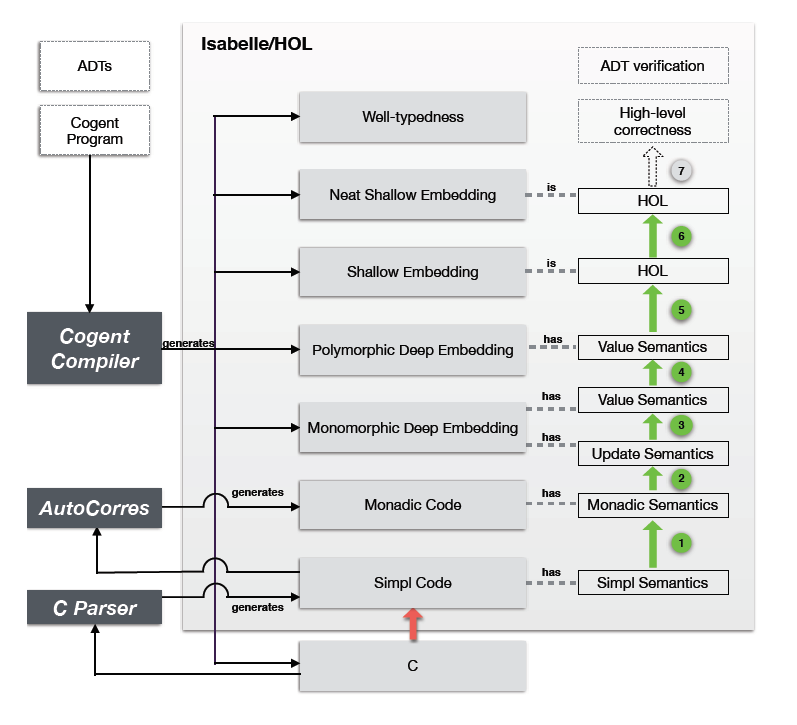
\includegraphics[height=18em]{fig/FIGURE_oconnor-2016_cogent-chain.PNG}}}$
    \end{column}
    \begin{column}{0.48\textwidth}
     %todo snippet of simplcode, or animation of translatin
      %$\vcenter{\hbox{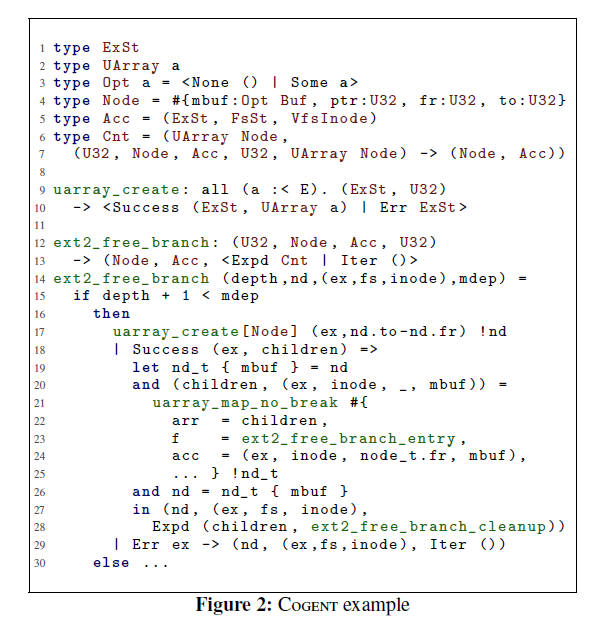
\includegraphics[height=18em]{fig/FIGURE_oconnor-2016_example.PNG}}}$
     \todo{Either some demonstration of translation or code snippet}
    \end{column}
  \end{columns}
\end{frame}

%\notes{
% Their verification chain is extensive.
%Given a $\cogent$ program, the $\cogent$ compiler first generates C code.
%A C parser then generates the semantics of this C code in Isabelle/Simpl (*A*).
%Using the Simple code, the /AutoCoress/ tool generates a monadic functional program (*B*).
%Then the $\cogent$ also produces the following representations:
%  - a monomorphic A-normal /deep/ embedding of the $\cogent$ program (*C*)
%  - a polymorphic A-normal /deep/ embeeded of the same (*D*)
%  - an A-normal /shallow/ embedding (*E*)
%  - a 'neat' /shallow/ embedding (syntactically close to $\cogent$ compiler input) (*F*)
%The chain of verification involves proving that the Simpl semantics (*A*) /refines/ the
%  monadic semantics (*B*), which /refines/ the update and value semantics of the monomorphic
%  deep embedding (*C*), which refines the value semantics of the polymorphic embedding (*D*),
%  which refines the HOL that is equal to the shallow embedding (*E*) and (*F*).
%Finally, user-supplied abstract datatypes (implemented in C) are verified according to the shallow embedding (*F*).
%The only unverified link the chain is output of the C-to-Isabelle parser that becomes Simpl code (*A*).
%
% kinds to determine is type can be freely shared or discarded
%}

% TODO maybe include
%$\vcenter{\hbox{\includegraphics[height=8em]{fig/FIGURE_oconnor-2016_shallow.PNG}}}$

\begin{frame}{COGENT: Not for Faint of Heart}
Work
    \begin{itemize}
        % so you get a guage of the work here
        \item 33.5 person-months for proof-automation
        \item 10 person-months engineering the compiler
        \item 18 person-months for design, formalization, and proof its properties
        \item 17 kLOC lines of Isabelle theorem prover code
        \item 9.5 kLOC of Haskell $\textsc{cogent}$ compiler code
        \item 6.5 kLOC of ext2 $\textsc{cogent}$ code $\Rightarrow$ 76.7 kLOC of Isabelle/HOL% proofs/embeddings
        \item A good way forward (embedded low-level DSLs combined with theorem proving)
    \end{itemize}
\end{frame}

% TODO shorten all of these
\begin{frame}{Other Linear Types}
  Typestate \footcite{strom_typestate:_1986}
    \begin{itemize}
        \item Avoid nonsensical execution sequences statically (using uninitialized value)
        \item Typestate is static invariant of each variable name at program point % i.e. need to merge control-paths, regardless of path to get to point
        \item Define a lattice of states and typestate transition system between them
        \item Linear types help because of restricting pointer assignment (1-1 mapping between variable names and run-time objects)
    \end{itemize}

  Quasi-linear types \footcite{kobayashi_quasi-linear_1999} % relaxtes linear type strong condition
    \begin{itemize}
        %\item Relax linear type strong condition
        \item Distinguish between consumed values vs those that may be returned
        \item Use $\kappa$ to control how often a variable of type $\tau^{\kappa}$ is used
        \item $\kappa = \delta$: accessed many times \emph{locally}, cannot be returned
%        \item Inspired $\textsc{paclang}$
%            \begin{itemize}
%                \item 0: not used at all
%                \item 1: value accessed at most once
%                \item $\omega$: accessed arbitrary number of times
%                \item $\delta$: accessed many times \emph{locally}, cannot be returned with result
%            \end{itemize}
        %\item Quasi-linear value (1) accessed as $\delta$ and then strictly as linear
        %\item Inspired PacLang
    \end{itemize}
    \vspace{0.1in}
\end{frame}

\begin{frame}{Other Linear Types}
\footnotesize
  Vault \footcite{deline_enforcing_2001} % TODO review this, TODO where is best place to put this, it combines typestate with regions like Cyclone...
    \vspace{-0.09in}
    \begin{itemize}
        \item Keys associate static capabilities with run-time resources, held-key set, type guards
        \item Functions annotated with effect clause (pre- and post-conditions on held-key set contents)
        %\item Freed regions before leaving scope % todo review
        %\item Types enforce code must free a region % todo review
        %\item static enforcement of various protocols
        \item Restrict aliasing, tracks fine-grained effects (requires more annotations)
        \item Catches Windows 2000 locking errors, IRP ownership model corresponds to tracked types
        % IRP = I/O Request Packets
        % todo add example?
    \end{itemize}
  Ordered types for memory layout \footcite{petersen_type_2003}
    \vspace{-0.09in}
    \begin{itemize}
        \item Restrict linear types (remove exchange property)
        \item Variables cannot change position $\Rightarrow$ locations in memory
        \item ``Orderly lambda calculus'' for size-preserving memory operations
        \item Coercions to manipulate ordered variables in frontier (combine/split to treat as different types)
    \end{itemize}
  \vspace{0.1in}
\end{frame}

\begin{frame}{Ownership}
\footnotesize
Ownership
    \begin{itemize}
      \item Every object has a unique owner
      \item Type include owner's name, accessing an object requires naming its owner
      % \item Involves work on aliasing
    \end{itemize}
  LCL \footcite{evans_static_1996}
    \vspace{-0.1in}
    \begin{itemize}
        \item $\texttt{owned}$ annotation to denote reference with obligation to release storage
        \item $\texttt{dependent}$ annotation for sharing; user ensures lifetimes contained properly % lifetime of dependent is within lifetime of owner
    \end{itemize}
  Ownership for Alias Protection \footcite{clarke_ownership_1998}
    \vspace{-0.1in}
    \begin{itemize}
      \item Two variables having ownership types with different declared object contexts cannot refer to same part of store, are not aliases
    \end{itemize}
  Races and deadlocks \footcite{boyapati_ownership_2002}
    \vspace{-0.1in}
    \begin{itemize}
      \item The lock protecting object also protects encapsulated objects
    \end{itemize}
  Singularity \footcite{fahndrich_language_2006}
    \vspace{-0.1in}
    \begin{itemize}
        \item Type system tracks resources, pass ownership of block to callee, possibly permanently
    \end{itemize}
  \vspace{0.1in}
\end{frame}

% what rust's type system is based on
\begin{frame}{Some Practical Affine Types}
  Alms \footcite{tov_practical_2011}
    \begin{itemize}
        \item Practical and general purpose
        \item Affine types: a \emph{weakening} of linear types: can drop but not duplicate
        \item Affine capabilities: separate a read-only reference to array from an affine writeable reference
        \item Define $^{a}\lambda_{ms}$ (based on System $F^{\omega}_{<:}$) and proof of soundness \note{types are maintained during evaluation, assuming no divergence}
        \item Implemented a capability-based interface to Berkeley sockets
        %TODO have they used it for memory management?
    \end{itemize}
\end{frame}

% TODO fix
\begin{frame}{Rust}
    % a conglomeration of all these topics
    Rust \footcite{matsakis_rust_2014} \ \footcite{jung_rustbelt:_2017}
%\begin{columns}[T]
%\begin{column}{0.52\textwidth}
%\begin{lstlisting}[
%    language=Rust,numbers=left,mathescape,basicstyle={\small\ttfamily}]
%let x = Foo::new();
%let y = x;
%printf("{}", x);
%\end{lstlisting}
%
%\pause
%
%\begin{lstlisting}[
%    language=Rust,numbers=left,mathescape,basicstyle={\small\ttfamily}]
%let x = Foo::new();
%let y = x;
%printf("{}", x);
%\end{lstlisting}
    \begin{itemize}
        \item Ownership \note{every value has uniquer owner}
        \item Lifetimes
        \item Type system enforces that objects have unique \alert{owners}
        \item Objects may be borrowed, obey lexical scope; borrows do not live longer than owner \note{like regions}
        \item Owner leaves scope $\Rightarrow$ object \alert{deallocated}
        \item One \alert{unique} mutable borrows, or multiple immutable borrows % solves aliasing
        \item $\texttt{unsafe}$ keyword for separating worlds %(i.e. Checked C's checked regions, Cogent) % TODO mention Cogent?!
%        \item Improves on Cogent b/c recursion, iteration, borrowing, mutable state
    \end{itemize}
\end{frame}
\note[itemize]{
\item performing certain actions on a resource (reading and writing a memory location) should require a 'right' 
\item or capability that is uniquely owned by one alias at any point during the execution of the program.
\item although right is uniquly owned, it cn be transferred from one alias to another
\item can be shared in a controlled manner
}

\begin{frame}{A Rust OS}
Rust OS \footcite{levy_ownership_2015}
    \begin{itemize}
        \item Ownership \emph{hinders} resource sharing
        \item AMM not optimized for HW resources/device drivers?
        \item Closures' req for dynamic memory is bad for embedded systems
    \end{itemize}
\todo{another attempt}
\end{frame}

\begin{frame}{Quick Temporal Recap}
    \begin{itemize}
      \item Capabilities and pointer-based metadata \note{can leverage info from spatial techniques to get full temporal safety}
      \item Regions \note{look toward effect types as an alternative to GC}
      \item Linear types \note{deallocate after use}
      \item Ownership and borrowing \note{unique owners help determine who is in charge, prevent data races, responsibility for cleaning}
    \end{itemize}
\end{frame}

\begin{frame}{Conclusion}
    \begin{itemize}[<+->]
        \item Memory errors $\Rightarrow$ \emph{type errors}
        \item \emph{Static} automatic memory management % like stack-based approach, important for embedded systems
        \item Be reasonable \uncover{and optimistic} % dynamic approaches still needed, static has come a long way
    \end{itemize}
\end{frame}

\begin{frame}{Thanks}
    \begin{center}
        \Huge{Thanks!}
    \end{center}
\end{frame}

%\subsection{Extra Slides}
%\begin{frame}{Hardware and Other Support for Spatial Safety}
%\begin{itemize}
% spin os
% \footcite:cha_retos:_2007 
%    \footcite{fullcite:kowshik_ensuring_2002} <---------- (at least in passing) (Control-C)
%    \footcite{fullcite:dhurjati_memory_2003}
%    \item \footcite{arora_architectural_2006}
%    \item \footcite{devietti_hardbound:_2008}
%    \item \footcite{binary compatible, low overhead}
%      % - can reduce overhead of CCured's SEQ and WILD pointers, array bounds checking in C#
%    \item \footcite{cowan_stackguard:_1998}
%     % - inserts canaries
%    \item \footcite{hasabnis_light-weight_2012}
%     % - guard zones with good performance
%    \footcite{kedia_simple_2017} %        -adding manual memory amangement to high-level langauges C#/java
% not sure where to include
%  \footcite:necula_proof-carrying_1997
%  \footcite:smith_sound_1998 
%  \footcite:siff_coping_1999 (physical subtyping, used by CCured)
%  seL4
%\end{itemize}
%\end{frame}

\begin{frame}{Alias Types}
  Alias types \footcite{smith_alias_2000}
    \begin{itemize}
        \item Problem: registers must be reused for data of different types constantly
        \item Aliasing constraints: describe shape of store; functions use to specify what they expect part of the store to look like
        \item Location and store polymorphism: dependence between pointer types and constraints, abstract away size/shape of store
        \item More expressive than linear: although aliasing constraints are linear, ptr values that flow through computation are not
        \item Constraint is mapping from locations to types; Pointer to location l has singleton type ptr(l)
    \end{itemize}
\end{frame}

\begin{frame}{Object-Based Temporal Safety}
\begin{itemize}
\item Mark locations which were de-allocated in shadow memory space (i.e. track a few bits of state for each byte in memory, indicating if location is currently valid)
\item Detect access of de-allocated locations
\item Fails if pointer points again to re-allocated space
\item Memcheck [30] 
    \begin{itemize}
      \item 10x slowdown
    \end{itemize}
\item Address Sanitizer: Serebryany "address santizier" 2012
    \begin{itemize}
        \item tripwire approach
        \item 73% slowdown
        \item can also detect small-stride buffer overflows
    \end{itemize}
\item Purify, valgrind
\end{itemize}
\end{frame}

\begin{frame}[fragile]{Extended Type Checking}
Extended Type Checking (ETC) \footcite{detlefs_overview_1995}
    \begin{itemize}
      \item use automatic theorem prover to detect index bounds in Modula-3
      \item use info in annotations to assist
      \item easier than C b/c no ptr arithmetic
    \end{itemize}
Also see: ETC/Java \footcite{flanagan_extended_2002}
\end{frame}

\begin{frame}[fragile]{LCLint}
LCLint \footcite{larochelle_statically_2001}
\begin{itemize}
    \item Leverage LCLint, an annotation-assisted buffer detection tool
    \item Annotations that constrain possible values a reference contains before/after funcall
    \item Function pre/post-condition with: $\footnotesize{\texttt{requires, ensures, unique, returned, modifies, out}}$ clauses
    \item Assumptions are $\texttt{minSet, maxSet, minRead, maxRead}$ % TODO put notes of what these mean, use in example below!!!
    \item Generates constraints at expression level, resolved w/ checking at statement level
    \item Heuristics to deal with loops nicely enough; neither sound nor complete
\end{itemize}
    Also see: ETC/Modula-3 \footcite{detlefs_overview_1995}, ETC/Java \footcite{flanagan_extended_2002}, CSSV \footcite{dor_cssv:_2003}
    \vspace{0.2in}
\end{frame}

\begin{frame}[fragile]{CSSV}
CSSV \footcite{dor_cssv:_2003}
\begin{itemize}
    \item Source-to-source translation
    \item Instruments program w/ additional variables describing string attrs
    \item Adds ~assert~ statements checking for unsafe string ops
    \item Statically analyze instr. version with \emph{integer analysis} to determine possible assertion failures
    \item Handles overlapping ptrs, etc.
    \item Disadv: \# vars in instr. quadratic in \# in orig.
\end{itemize}
    Also see: ETC/Modula-3 \footcite{detlefs_overview_1995}, LCLint \footcite{larochelle_statically_2001}, ETC/Java \footcite{flanagan_extended_2002}
    \vspace{0.2in}
\end{frame}
%- fullcite:bodik_abcd:_2002 <----
%- fullcite:wagner_first_2000 
%- disadv: proves correct fraction of array/ptr references (useful for reducing checks)

\end{document}

%%% Local Variables:
%%% mode: latex
%%% TeX-master: t
%%% TeX-engine: xetex
%%% End:
